%%%%%%%%%%%%%%%%%%%%%%%%%%%%%%%%%%%%%%%%%%%%%%%%%%%%%%%%%
%%%%%IMPORTS:

%packages a utilizar:
\documentclass{report}
\usepackage[T1]{fontenc}     % Fontes T1
\usepackage[utf8]{inputenc}  % Input UTF8
\usepackage[top=3cm,bottom=3cm,left=3cm,right=2.5cm,asymmetric]{geometry} %fronteiras
%\usepackage[nottoc]{tocbibind}
\usepackage[table]{xcolor} %Colorir tabelas
\usepackage[backend=biber, style=ieee]{biblatex} %bibliografia
\usepackage{csquotes}  % referências
\usepackage[portuguese]{babel} %Usar língua portuguesa
\usepackage{blindtext} 
\usepackage[printonlyused]{acronym}  %Acrónimos
\usepackage{hyperref}  %Autoref no índice
\usepackage{graphicx}  %Usar imagens
\usepackage{titling}
\usepackage{multicol} %multicoluna de texto
\usepackage{adjustbox}
\renewcommand{\figurename}{Fig.} 
\renewcommand{\tablename}{Tabela} 
\usepackage[font=small,tableposition=top]{caption} 
\usepackage[font=small]{subcaption}
\usepackage{xcolor} %cor nos textos
\usepackage{amsmath} %matematica
\usepackage{amssymb} %simbolos matematicos
\graphicspath{ {./images/} } %directorio das imagens
\usepackage{fancyhdr}
\usepackage{authblk}
\usepackage{float} %Posicionamento exacto das figuras no texto
\usepackage{url}   %referencias URL
\usepackage{blindtext}
\def\UrlBreaks{\do\/\do-} %não cortar referencias

\usepackage{indentfirst} %Garantir avanço do primeiro parágrafo
\hypersetup{pdfborder=0 0 0} %Remover a caixa vermelha das referências
\usepackage{chngcntr} %Numeração contínua das figuras
\counterwithout{figure}{chapter} %Numeração contínua de figuras
\counterwithout{table}{chapter} %Numeração contínnua de tabelas
\setlength{\parskip}{0.2cm} %Aumento de espaçamento entre parágrafos

\usepackage{hyperref}

 
\begin{document}	
	%Definições do Relatório

%Dados Gerais:
\def\titulo{Projecto Final: \\ Máquina de Lavagem de Roupa}
\def\data{Junho de 2022}
\def\versao{Ver.: 1.13}
\def\departamento{Departamento de Electrónica Telecomunicações e Informática}
\def\empresa{Universidade de Aveiro}
\def\logotipo{logotipo_ua.png}

%Dados dos Autores:
%primeiro autor:
\def\pautor{João Pedro Nunes Vieira} 
\def\numpautor{Nº Mec.:  50458}
\def\contactopautor{joaopvieira@ua.pt}
%segundo autor:
\def\sautor{Leandro Roque Costa} 
\def\numsautor{Nº Mec.: 110326}
\def\contactosautor{lrc@ua.pt}
%
\def\autores{\pautor \\ \sautor}

	%Capa do Relatório:
\begin{titlepage} 
	\begin{center}
	\includegraphics[scale=0.50]{\logotipo}
	\line(1,0){350} \\ 
		\vspace*{2mm}
	{\Large \uc} \\
		\vspace*{2mm} 	
	{\Huge \titulo} \\
		\vspace*{2mm}
	\line(1,0){350} \\ 
		\vspace*{2mm}
	{\Large \empresa} \\
		\vspace*{20mm}
	{\Large \autores} \\ 
		\vspace*{\fill}
	\end{center}

	\begin{flushright} 
		{\large \departamento} \\ 
		{\versao} 
	\end{flushright}

\end{titlepage}

	%Página de Título:
\predate{\begin{flushright}\small}
\postdate{\par\end{flushright}}

\title{ 
	{\huge\textbf{\titulo} } \\ 
	{\large \departamento\\ \empresa} }

\author{

    \begin{tabular}{l}
        \pautor, \numpautor\hfil \\
        \contactopautor
    \end{tabular}
    \and
    \begin{tabular}{l}
        \sautor, \numsautor\hfil \\
        \contactosautor
    \end{tabular}
    \and
    \begin{tabular}{l}
        \tautor, \numtautor\hfil \\
        \contactotautor
    \end{tabular}
    \and
    \begin{tabular}{l}
        \qautor, \numqautor\hfil \\
        \contactoqautor
    \end{tabular}
}




\date{\vspace{\fill}{\data}} 
\maketitle
	
%%%%%%%%%%%%%%%%%%%%%%%%%%%%%%%%%%%%%%%%%%%%%%%%%%%%%%%%%
%%%%%INDICE:

\renewcommand{\contentsname}{Conteúdos}
\tableofcontents
\listoffigures
\pagenumbering{roman}

%%%%%%%%%%%%%%%%%%%%%%%%%%%%%%%%%%%%%%%%%%%%%%%%%%%%%%%%%
%%%%%ACRÓNIMOS:

\chapter*{Acrónimos}
\begin{acronym}

\acro{ua}[UA]{Universidade de Aveiro}
\acro{leci}[LECI]{Licenciatura em Computadores e Informatica}
\acro{uc}[UC]{Unidade Curricular}
\acro{lsd}[LSD]{Laboratórios de Sistemas Digitais}
\acro{mux}[MUX]{Multiplexer}
\acro{dec}[DEC]{Decoder}
\acro{enc}[ENC]{Encoder}
\acro{vhdl}[VHDL]{Very high speed integrated circuits Hardware Description Language}
\acro{i/o}[Portos E/S]{Portos de Entrada e Saída}
\acro{cau}[CaUs]{Casos de Utilização}
\acro{mef}[MEF]{Máquina de Estados Finitos}
\acro{mlr}[MLR]{Máquina de Lavar Roupa}
\acro{fpga}[FPGA]{Field-Programmable Gate Array}

\end{acronym}

%%%%%%%%%%%%%%%%%%%%%%%%%%%%%%%%%%%%%%%%%%%%%%%%%%%%%%%%%
%%%%%HEADERS & FOOTERS:

\pagestyle{fancy}
\fancyhf{}
\rhead{\titulo}
\lhead{Introdução}
\cfoot{\thepage}

%%%%%%%%%%%%%%%%%%%%%%%%%%%%%%%%%%%%%%%%%%%%%%%%%%%%%%%%%
%%%%%INTRODUÇÃO:


\chapter*{Introdução}
\label{chap.Intro}
\pagenumbering{arabic}
\begin{multicols}{2}

O presente relatório contempla o desenvolvimento geral do \textbf{Projeto Final} no âmbito da \ac{uc} \ac{lsd}, lecionada no decorrer do ano letivo 2021/22 na \ac{ua}. Foram utilizadas ferramentas e conhecimentos teóricos e práticos abordados no decorrer da \ac{uc}, nomeadamente o software \textit{Quartus Prime - Ver.20.1 - Lite Edition}. \\
O projeto consiste no planeamento, sintetização, modelação e validação de um sistema digital cujo objetivo principal é a modelação em \textbf{\ac{vhdl}} de uma \textbf{\ac{mlr}}, que deverá disponibilizar programas diferentes de funcionamento para a interação com o utilizador. \\

\end{multicols}

\section{Metodologia}
\label{sec.requisitos}
Foi adotado um sistema de desenvolvimento \textit{Agile}, onde primariamente foi executado o levantamento, identificação e especificação de requisitos funcionais, \ac{i/o} e \ac{cau}, usando como recurso base o \textbf{Guião Nº7} de \ac{lsd} atribuído a grupo de trabalho. Seguidamente foi feito o design geral do projeto bem como delineação de estados para a \ac{mef}. Finalmente a partir do design e da \ac{mef} delineados, foram desenvolvidos sequencialmente os componentes, sendo cada um testado e melhorado ao longo do tempo, por forma a que funcionassem corretamente e que o ficheiro \textit{TOP\_LEVEL} tivesse um funcionamento adequado e requerido.

%%%%%

\section{Especificação: Requisitos funcionais}
\label{sec.requisitos}

\textbf{NOTA IMPORTANTE:} Apenas será usado um único sinal de Clock (50Mhz) ou um divisor da frequência deste para sincronização de todos os componentes. 
	
\begin{table}[H]
	\centering
	\caption{Requisitos funcionais de entrada.}
	\begin{tabular}{|c|c|c|c|c|}\hline
	
		ID & Sinais de Entradas & Tipo & Condições \\ 
        \hline
        RE1 & Clock & 50Mhz & Único e Global \\
		RE2 & ON/OFF & 1 Botão Switch(SW) & Liga e Desliga toda a \ac{mlr}. \\	    
	    RE3 & Reset & 1 Botão Switch(SW) & Reinicia todos os componentes da \ac{mlr} (sincrono) \\ 
		RE4 & Porta da Máquina & 1 Botão Switch(SW) & Entrada door: \ac{mlr} não inicia se estiver aberta. \\
		RE5 & Start & 1 Botão Switch(SW) & Inicia programa selecionado    \\
	    RE6 & Programa & 2 Botões Switch(SW) & Seleção de programa pretendido   \\
    \hline
    \end{tabular}
    \label{tab.req_funcionais_entrada}
\end{table}	

\textbf{NOTA - RE3:} Deve aparecer letra \textbf{"P"} no display BCD (\autoref{chap.arquitetura}).\\

	
\begin{table}[H]
	\centering
	\caption{Requisitos funcionais de saida.}
	\begin{tabular}{|c|c|c|c|c|}\hline
	
		ID & Sinais de Entradas & Tipo & Condições \\ 
        \hline
        RS1 & ON/OFF & LEDR & Indicação de \ac{mlr} ligada/desligada. \\
		RS2 & Programa & Display BCD 7 Segmentos & Indica programa selecionado. \ac{mlr}. \\	    
	    RS3 & Letra "P" & Display BCD 7 Segmentos & Ler: RE3 e nota anterior. \\ 
		RS4 & Tempo de cada estado & Display BCD 7 Segmentos & Deve mostrar \textbf{"="} caso \ac{mlr} parada.  \\
		
    \hline
    \end{tabular}
    \label{tab.req_funcionais_saida}
\end{table}	

\begin{table}[H]
	\centering
	\caption{Tabela de Operações(S.) e tempo requerido(segundos):}
	\begin{tabular}{|c|c|c|c|c|c|c|c|c|c|c|c|}\hline

		Estado associado & Operação 		& Sinal    	  & Tempo(s) 	\\ 
        \hline		
		S0				 & IDLE				& N/A		  & 0s		\\
		\hline		
		S1				 & Meter água		& water valve & 7s 		\\
		\hline		
		S2				 & Enxaguar			& water pump  & 10s		\\
		\hline		
		S3				 & Retirar água		& rinse		  & 4s		\\
		\hline		
		S4				 & Centrifugação	& spin		  & 5s		\\
		\hline
		S5				 & Fim				& finish	  & 2s		\\
		\hline
    \end{tabular}
    \
    \label{tab.estados}
\end{table}	

%%%%%%%%%%%%%%%%%%%%%%%%%%%%%%%%%%%%%%%%%%%%%%%%%%%%%%%%%
%%%%%CAPÍTULO 1: Arquitetura do Sistema

\chapter{Arquitetura do Sistema}	
\label{chap.arquitetura}
\lhead{Arquitetura}

%%%%%

\section{Componentes:}
\label{sec.comp}

O projeto contem 9 componentes desenvolvidos em VHDL, para instanciação e elaboração do componente \textit{TOP\_LEVEL}. 
	\begin{enumerate}
	
		\item\textbf{ControlPanel:} Componente \textit{"register"} que controla os portos de entrada principais da \ac{mlr} e os sincroniza, por forma a evitar inconsistências de estado do sistema no caso de mudança de um sinal lógico de entrada muito perto de uma transição ativa de relógio.

		\item\textbf{WashingFSM:} \acf{mef}, que define e controla os estados finitos internos da \ac{mlr} bem como os seus sinais internos, outputs e transições de estados.

		\item\textbf{Timer:} Componente do tipo \textit{"counter"} que após receção de um valor de tempo pedido pela \ac{mef}, incrementa um valor temporal binário até que igualdade seja estabelecida onde a contagem é parada e feito o envio output de um sinal para mudança de estado - sinal de porta \textit{"change"}.

		\item\textbf{Pulser:} Ligado ao componente \textit{"Timer"}, ativa um sinal uma vez por segundo - frequência: 1hz.
		\item\textbf{TimerRegister:} componente do tipo \textit{"register"} que regista os sinais de tempo decorrido de saida do componente \textit{"timer"} e os redireciona para dentro do mesmo, evitando a criação de latches automáticas.
		
		\item\textbf{RMan:} Abreviatura para \textit{"RegisterManager"}, é um componente do tipo \textit{"register"} que regista os sinais de \textit{"reset"} (global e de saida do componente \textit{"TimerRegister"}, e gere qual deles deve ser ativado para dar entrada no componente \textit{"timer"}.

		\item\textbf{JumpRegister:} componente do tipo \textit{"register"} que regista os sinais de repetição de saida do componente \textit{"WashingFSM"} e os redireciona para dentro do mesmo, evitando a criação de latches automáticas.
		
		\item\textbf{Bin7SegDec\_Timer:} \textit{Decoder} Binário de 7 Segmentos que executa o display do tempo decorrido em cada estado da \ac{mef}, até que executado uma operação de mudança de estado.

		\item\textbf{Bin7SegDecProg:} \textit{Decoder} Binário de 7 Segmentos que executa o display do programa de lavagem selecionado.

		\item\textbf{Bin7SegDecProg:} \textit{Decoder} Binário de 7 Segmentos que executa o display do programa de lavagem selecionado.
		
		\item\textbf{WashingMachine - (TOP\_LEVEL):} Componente \textit{"Top-Level"} do projecto, criado através da instanciação sequencial adequada dos componentes anteriormente descritos.
		
	\end{enumerate}


\begin{figure}[H]
	\centering
	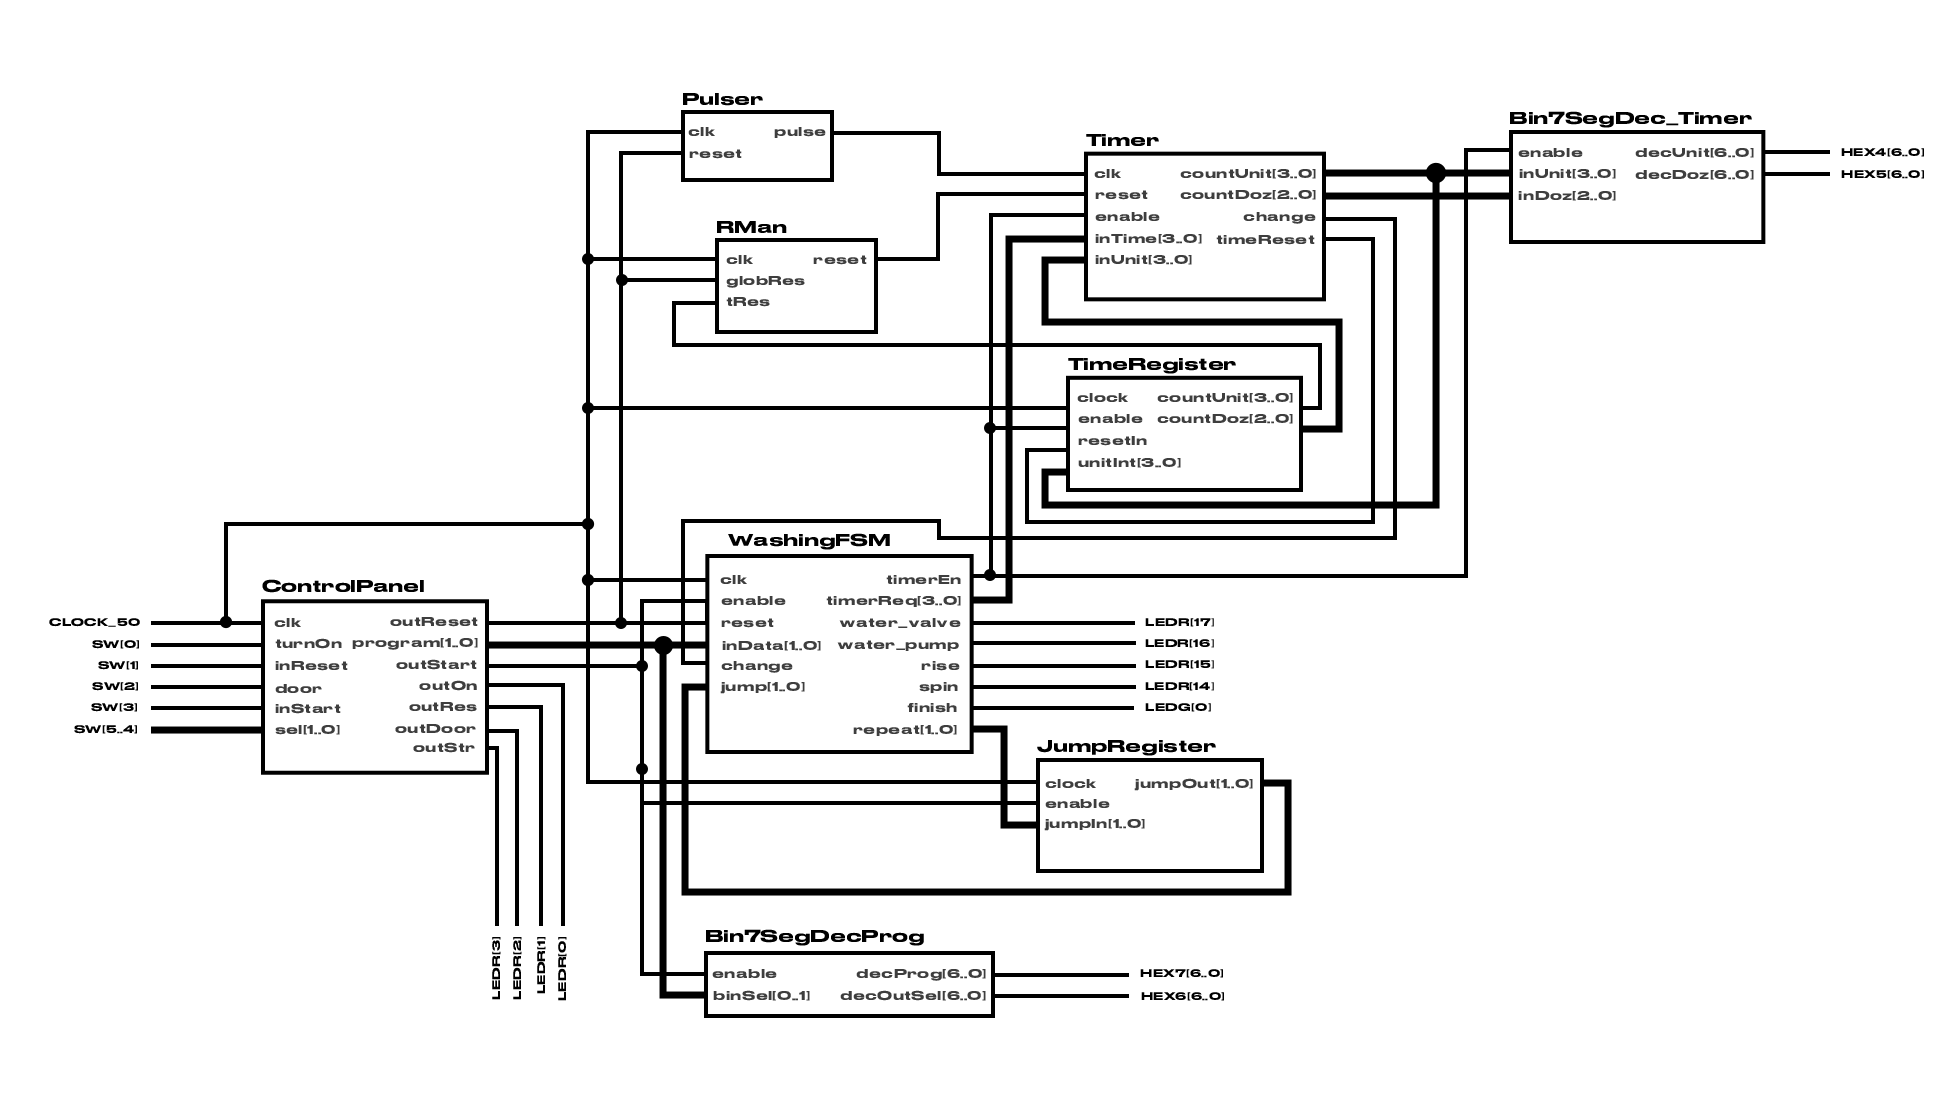
\includegraphics[width=18cm]{ArquiteturaSemFundo.png}
	\caption{Diagrama de Blocos da Arquitetura do Sistema\\}
	\label{fig:diag_blocos}
\end{figure} 

%%%%%

\newpage
\section{Diagrama de Estados:}
\label{sec.diag_estados}


Devido à necessidade de um utilizador executar uma pré-lavagem, antes de uma lavagem completa, foi adotado um sistema de seleção de operações baseada em \textit{grey-code}, no qual a diferença de bits entre as operações (estados finitos da \ac{mef}) seja de uma unidade binária, fazendo a troca entre programas fácil e intuitiva, já que iremos apenas usar \textit{switches} para a seleção dos mesmos. \\
Por forma a implementar uma \acf{mef}, foi elaborada um diagrama de estados do qual resulta a tabela de estados e configurações seguintes : 


\begin{figure}[H]
	\centering
	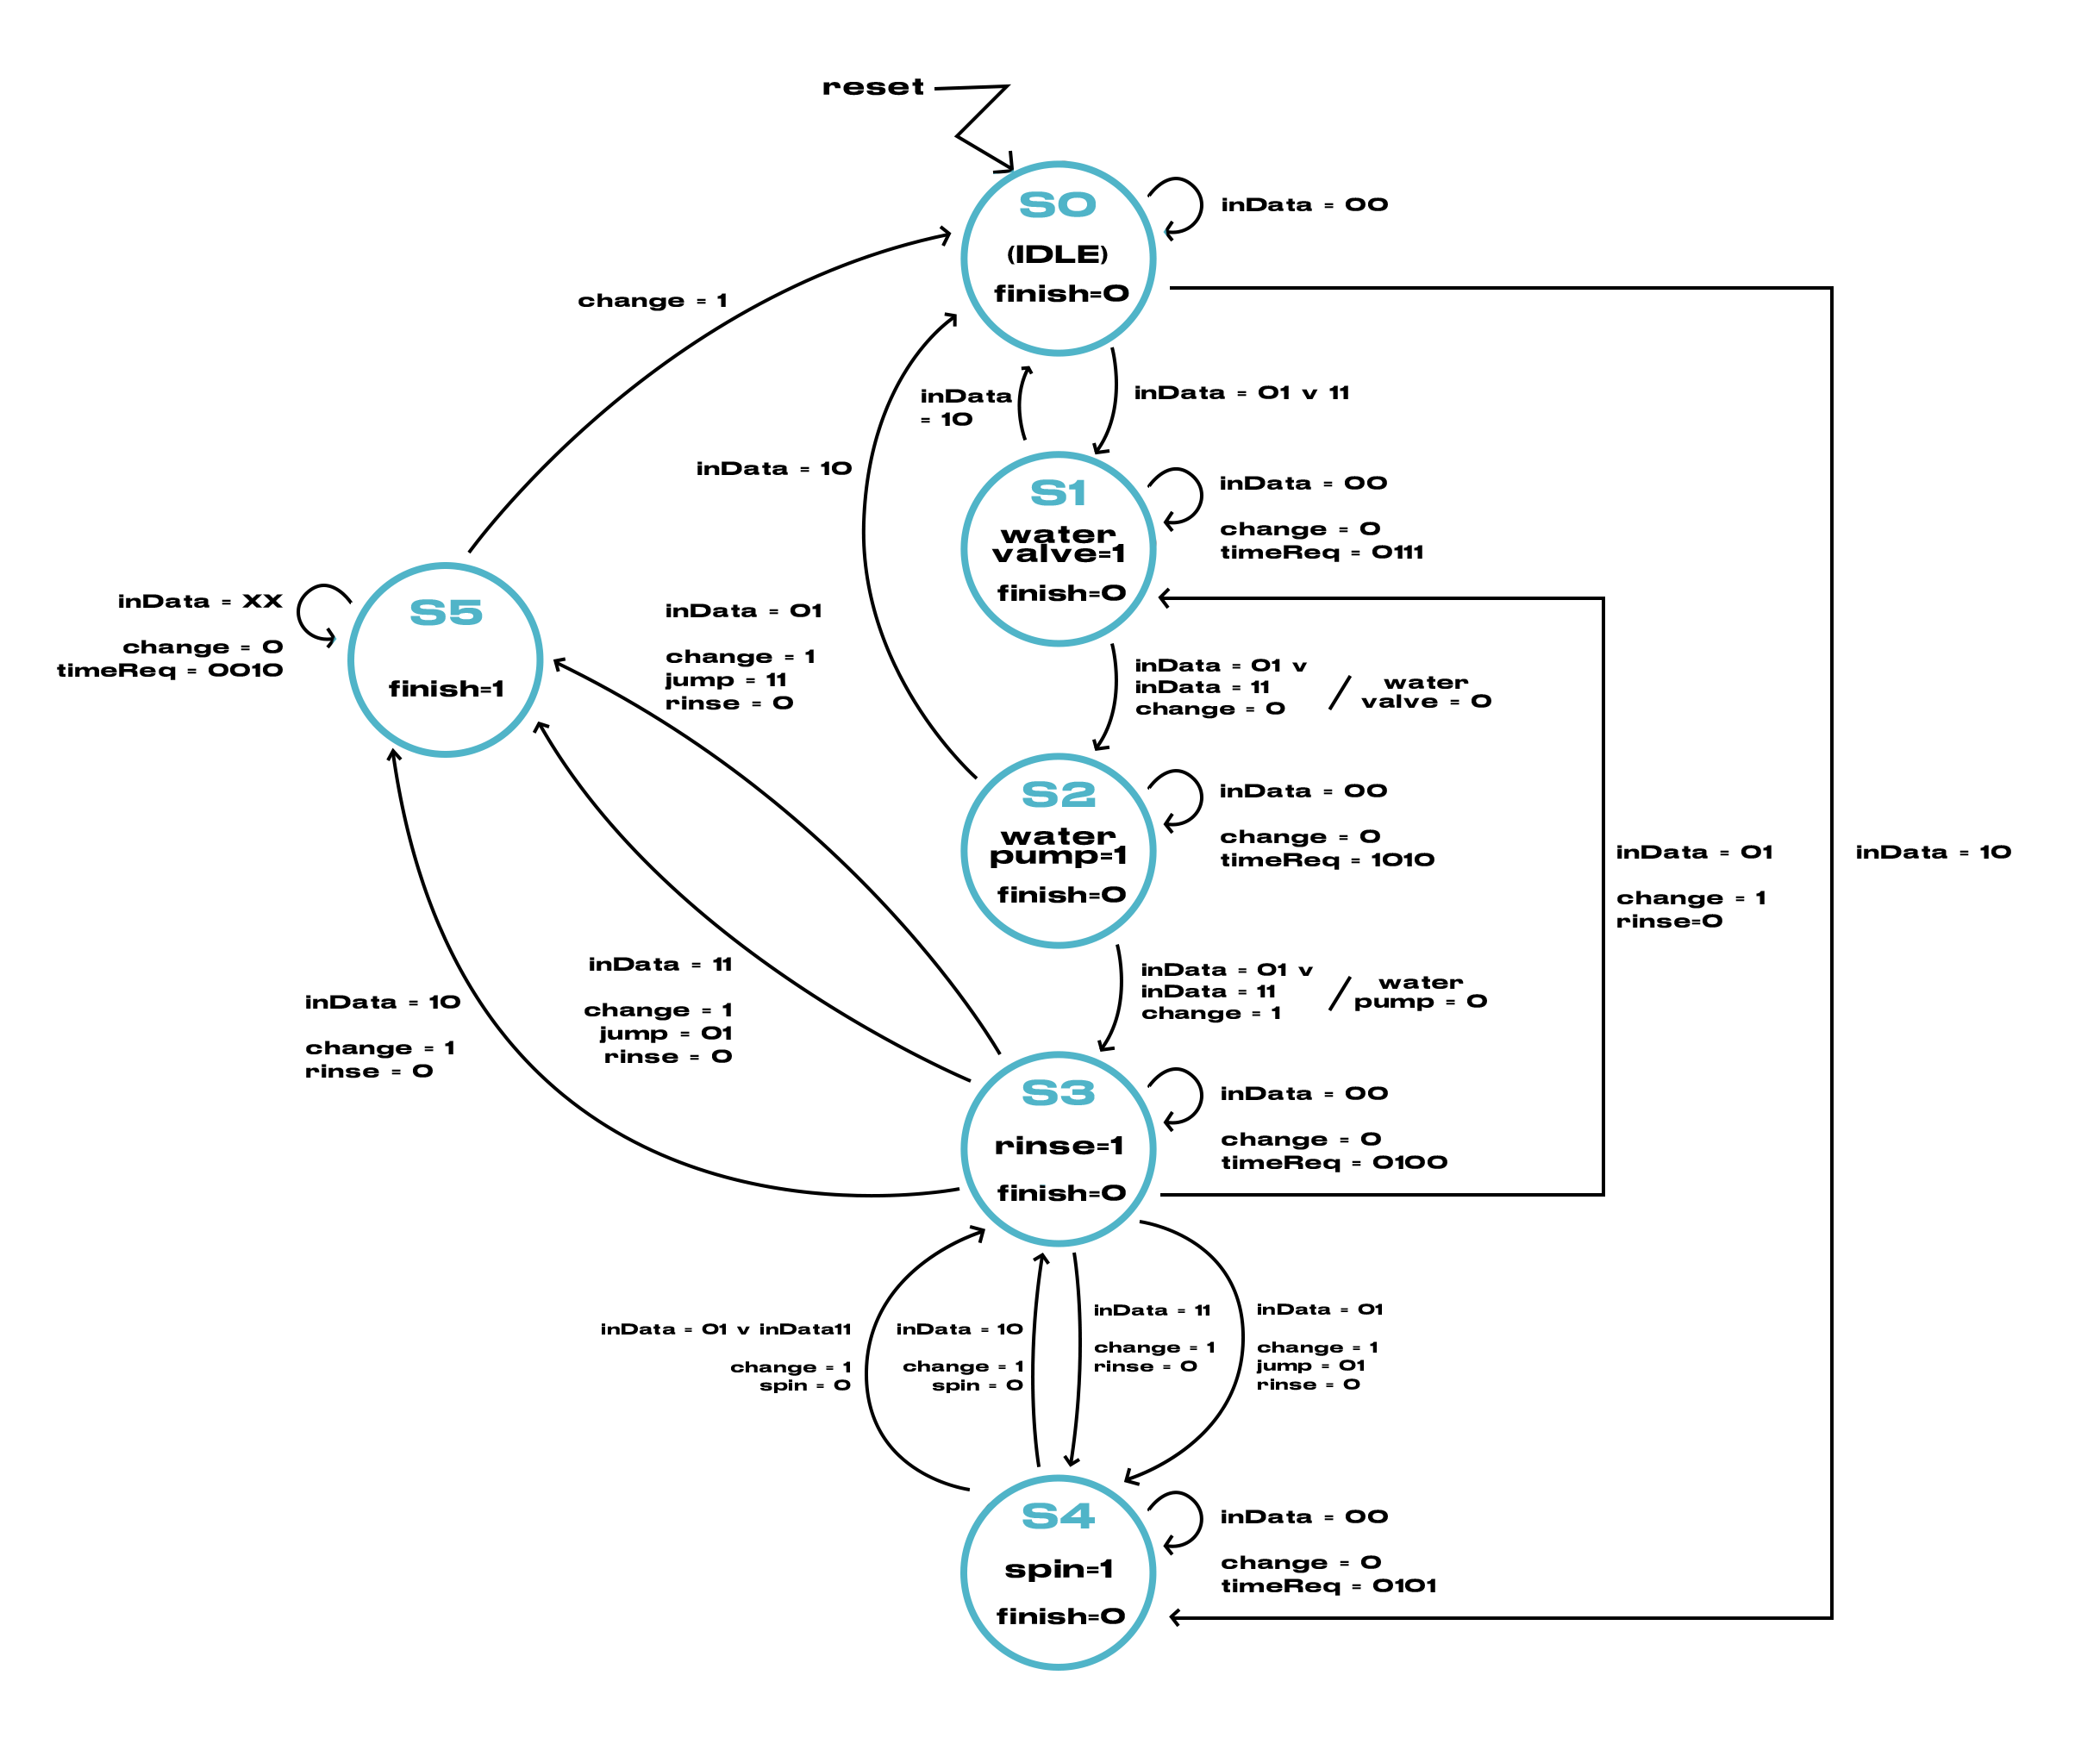
\includegraphics[width=17cm]{DiagramaSemFundo.png}
	\caption{Diagrama de Estados \\}
	\label{fig:diag_blocos_bdf}
\end{figure} 

\begin{table}[H]
	\footnotesize
	\centering
	\caption{Tabela de Programas de Lavagem, Operações(S.):}
	\begin{tabular}{|c|c|c|c|c|c|c|c|c|c|c|c|}\hline

		Programa 			  & Input Selecionado & Sequencia de Operações 				& Tempo Total \\ 
        \hline		
		Nº1: Lavagem completa & 		01        & S1->S2->S3->S1->S2->S3->S4->S3->S5	& 53 segundos \\
        \hline
        Nº2: Pré-lavagem 	  &         11 	      & S1->S2->S3->S4->S3->S5    			& 32 segundos \\
		\hline
        Nº3: Extra-Spin 	  &         10 	      & S4->S3->S5			    			& 11 segundos \\
		\hline
    \end{tabular}
    \
    \label{tab.estados}
\end{table}	
\normalsize

\begin{table}[H]
	\footnotesize
	\centering
	\caption{Tabela de Estados:}
	\begin{tabular}{|c|c|c|c|c|c|c|c|c|c|c|c|}\hline
	
				& Input	 & Input  & Input  & Output	 & 		   & Output		 & Output 	  & Output & Output & Output \\
        \hline		
		pState 	& inData & jump   & change & timeReq & nState  & valve & pump & rinse & spin & finish 	\\ 
        \hline
        S0 		& 00 	 & xx 	  & x		& 0000	 & S0      & 0     	     & 0 	      & 0	  & 0    & 0 	 	\\
		S0 		& 01 	 & xx 	  & x		& 0000	 & S1 	   & 0 	   	     & 0 	      & 0 	  & 0    & 0	 	\\
        S0 		& 10 	 & xx 	  & x		& 0000	 & S4      & 0     	     & 0 	      & 0	  & 0    & 0 	 	\\
        S0 		& 11 	 & xx 	  & x		& 0000	 & S1      & 0     	     & 0 	      & 0	  & 0    & 0 	 	\\
		\hline		
		S1 		& xx 	 & xx 	  & 0		& 0111	 & S1      & 1     	     & 0 	      & 0	  & 0    & 0 	 	\\
		S1 		& 00 	 & xx 	  & 1		& 0000	 & S1      & 0     	     & 0 	      & 0	  & 0    & 0 	 	\\
		S1 		& 01 	 & xx 	  & 1		& 0000	 & S2      & 0     	     & 0 	      & 0	  & 0    & 0 	 	\\
		S1 		& 10 	 & xx 	  & 1		& 0000	 & S0      & 0     	     & 0 	      & 0	  & 0    & 0 	 	\\
		S1 		& 11 	 & xx 	  & 1		& 0000	 & S2      & 0     	     & 0 	      & 0	  & 0    & 0 	 	\\
		\hline		
		S2 		& xx 	 & xx 	  & 0		& 1010	 & S2      & 0     	     & 1 	      & 0	  & 0    & 0 	 	\\
		S2 		& 00 	 & xx 	  & 1		& 0000	 & S2      & 0     	     & 0 	      & 0	  & 0    & 0 	 	\\
		S2 		& 01 	 & xx 	  & 1		& 0000	 & S3      & 0     	     & 0 	      & 0	  & 0    & 0 	 	\\
		S2 		& 10 	 & xx 	  & 1		& 0000	 & S0      & 0     	     & 0 	      & 0	  & 0    & 0 	 	\\
		S2 		& 11 	 & xx 	  & 1		& 0000	 & S3      & 0     	     & 0 	      & 0	  & 0    & 0 	 	\\
		\hline
		S3 		& xx 	 & xx 	  & 0		& 0100	 & S3      & 0     	     & 0 	      & 1	  & 0    & 0 	 	\\
		S3 		& 00 	 & xx 	  & 1		& 0000	 & S3      & 0     	     & 0 	      & 0	  & 0    & 0 	 	\\
		S3 		& 01 	 & 00 	  & 1		& 0000	 & S1      & 0     	     & 0 	      & 0	  & 0    & 0 	 	\\
		S3 		& 01 	 & 01 	  & 1		& 0000	 & S4      & 0     	     & 0 	      & 0	  & 0    & 0 	 	\\
		S3 		& 01 	 & 10 	  & 1		& 0000	 & S1      & 0     	     & 0 	      & 0	  & 0    & 0 	 	\\
		S3 		& 01 	 & 11 	  & 1		& 0000	 & S5      & 0     	     & 0 	      & 0	  & 0    & 0 	 	\\		
		S3 		& 10 	 & xx 	  & 1		& 0000	 & S5      & 0     	     & 0 	      & 0	  & 0    & 0 	 	\\
		S3 		& 11 	 & 00 	  & 1		& 0000	 & S4      & 0     	     & 0 	      & 0	  & 0    & 0 	 	\\
		S3 		& 11 	 & 01 	  & 1		& 0000	 & S5      & 0     	     & 0 	      & 0	  & 0    & 0 	 	\\
		S3 		& 11 	 & 10 	  & 1		& 0000	 & S4      & 0     	     & 0 	      & 0	  & 0    & 0 	 	\\
		S3 		& 11 	 & 11 	  & 1		& 0000	 & S4      & 0     	     & 0 	      & 0	  & 0    & 0 	 	\\
		\hline
		S4 		& xx 	 & xx 	  & 0		& 0101	 & S4      & 0     	     & 0 	      & 0	  & 1    & 0 	 	\\
		S4 		& 00 	 & xx 	  & 1		& 0000	 & S4      & 0     	     & 0 	      & 0	  & 0    & 0 	 	\\
		S4 		& 01 	 & xx 	  & 1		& 0000	 & S3      & 0     	     & 0 	      & 0	  & 0    & 0 	 	\\
		S4 		& 10 	 & xx 	  & 1		& 0000	 & S3      & 0     	     & 0 	      & 0	  & 0    & 0 	 	\\
		S4 		& 11 	 & xx 	  & 1		& 0000	 & S3      & 0     	     & 0 	      & 0	  & 0    & 0 	 	\\
		\hline
		S5 		& xx 	 & xx 	  & 0		& 0010	 & S5      & 0     	     & 0 	      & 0	  & 0    & 1 	 	\\
		S5 		& xx 	 & xx 	  & 1		& 0000	 & S0      & 0     	     & 0 	      & 0	  & 0    & 0 	 	\\
		\hline
		
    \end{tabular}
    \label{tab.estados}
\end{table}	
\normalsize


%%%%%%%%%%%%%%%%%%%%%%%%%%%%%%%%%%%%%%%%%%%%%%%%%%%%%%%%%
%%%%%CAPÍTULO 2: Implementação

\chapter{Implementação}	
\label{chap.implementação}
\lhead{Arquitetura}

A implementação deste projeto seguiu uma metodologia estratégica faseada nas seguintes \textbf{7 fazes}:

%%%%%

\section{Fase 1}
\label{sec.fase1}

Tal como referido no \autoref{chap.arquitetura} nas \autoref{sec.comp} e \autoref{sec.diag_estados}, foi implementada uma \ac{mef} que gera sinais de saída que controlam sequencialmente as diferentes funções (operações) da \acf{mlr}, para cada um dos programas selecionados (\autoref{sec.programas}), mediante as entradas dos \ac{i/o}, gerando ainda sinais de controlo de um temporizador (componente \textit{Timer}). \\

%%%%%
\subsection{Sinais de Entrada/Saída:} 
\label{sec.IO_FSM}
\begin{itemize}

	\item\textbf{clock:} Sinal de clock global e único de 50Mhz.
	\item\textbf{enable:} Sinal que dá permissão para a iniciação do funcionamento da máquina de lavar roupa.
	\item\textbf{reset:} Sinal que permite reiniciar a \acf{mlr}.	
	\item\textbf{inData:} Sinal que	transmite o programa selecionado pelo utilizador.
	\item\textbf{change:} Sinal de entrada, redirecionado do componente \textit{Timer} que controla a mudança de estado da \ac{mef}.
	\item\textbf{jump:} Sinal que indica qual o estado subsequente ao estado atual. 
	
	
	\item \textbf{timeEn:} Sinal de saída de controlo de inicio da contagem do um temporizador para o tempo requerido.	
		\item \textbf{timerReq:} \textit{"timer request"}, é um sinal de saída de 4 bits que requisita ao temporizador (\textit{Timer}) um valor temporal  para contar em segundos para execução da operação/função pretendida.
	\item\textbf{water\_valve:} Sinal de saída para atuar sobre a válvula de admissão de água.
	\item\textbf{water\_pump:} Sinal de saída para ligar a bomba de água.
	\item\textbf{rinse:} Sinal de saída para a execução de enxaguamento de roupa.
	\item\textbf{spin:} Sinal de saída para controlar a velocidade do tambor, executando centrifugação (ie, retira o excesso de água da roupa.
	\item\textbf{finish:} Sinal de saída que indica o fim da execução do programa selecionado.	 
	 
\end{itemize}

\begin{figure}[H]
	\centering
	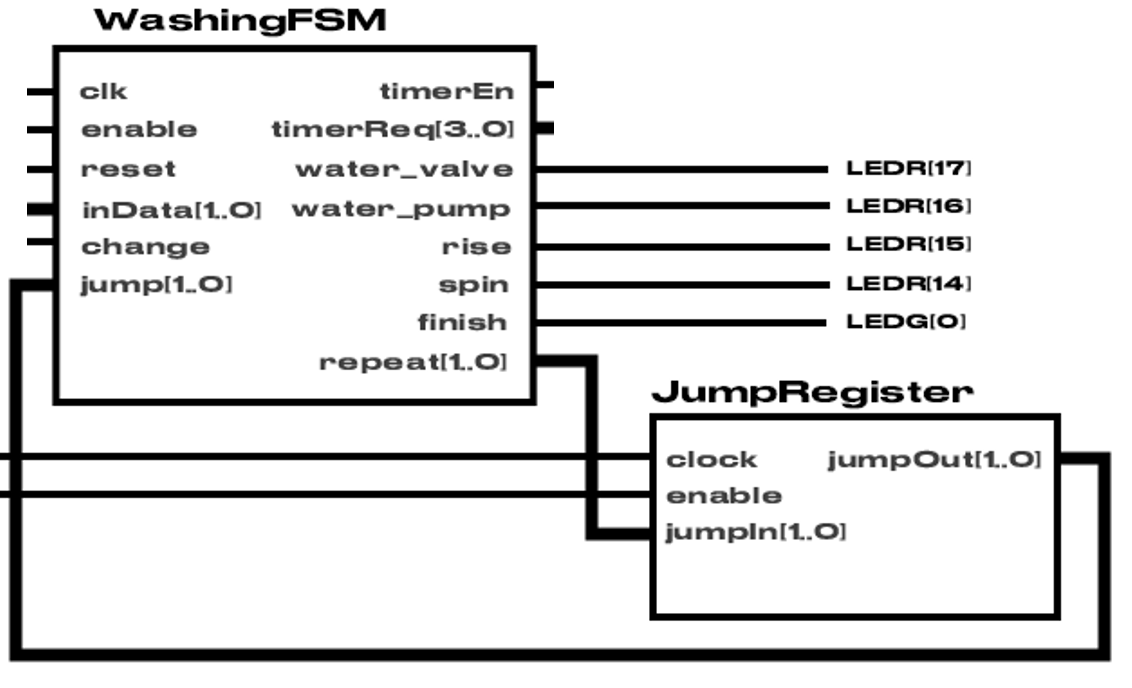
\includegraphics[width=10cm]{WashingFSM.png}
	\caption{\acf{mef} \\}
	\label{fig:WashingFSM}
\end{figure} 

%%%%%
\section{Fase 2}
\label{sec.fase2}

Tal como referido no \autoref{chap.arquitetura} na \autoref{sec.comp}, foi implementado um temporizador (componente \textit{Timer}) que conta o tempo decorrido em cada estado (e consequentemente o tempo de funcionamento da operação) e controla a mudança de estado da \ac{mef} após completar esse mesmo tempo, recebendo e enviando os seguintes sinais:

\subsection{Sinais de Entrada/Saída:} 
\label{sec.IO_Timer}
\begin{itemize}

	\item\textbf{clock:} Sinal de entrada que recebe uma ativação (pulso) do componente \textit{Pulser} (frequência: 1hz), permitindo assim que a contagem seja executada num tempo de 1 unidade por cada segundo de tempo real .
	
	\item\textbf{reset:} Sinal de entrada rececionado do componente \textit{RMan}, que permite recetar o temporizador para valores iniciais.
	
	\item\textbf{enable:} Sinal de entrada que dá permissão para a iniciação do processo de contagem do temporizador.
	
	\item\textbf{inTime:} Sinal de entrada de 4 bits, que é receciado da \ac{mef} \autoref{sec.IO_FSM}. Este sinal, indica o tempo a contar requisitado pelo estado finito para o decorrer da operação associada ao mesmo.
	
	\item\textbf{inUnit:} Sinal de entrada de 4 bits rececionado do componente de registo \textit{TimeRegister}. Este sinal indica se a contagem a ser executada pelo \textit{Timer} é igual ao tempo requisitado pelo sinal anterior (inTime). Caso sejam iguais, o temporizador termina a sua contagem e envia à \ac{mef} um sinal (\textit{change}) de ativação para mudança do estado (fim de operação atual).
	
	\item\textbf{change:} Sinal de saída referido no ponto anterior que controla a mudança de estado finito interno da \ac{mef}.
	
	\item\textbf{countUnit:} Sinal de saída de 4 bits, que indica os valores de tempo de 0(Zero) até 9(Nove) em unidades, para conversão em visualização (display) em sistema decimal.
	
	\item\textbf{countDoz:} Sinal de saída de 4 bits, que indica os valores de tempo de 1(Zero) até 7(Sete) em dezenas, para conversão em visualização (display) em sistema decimal.
	
	\item\textbf{timeReset:} Sinal de saída que indica ao componente \textit{TimeRegister} que deve ser executado uma operação \textit{reset} ao temporizador.

\end{itemize}

\begin{figure}[H]
	\centering
	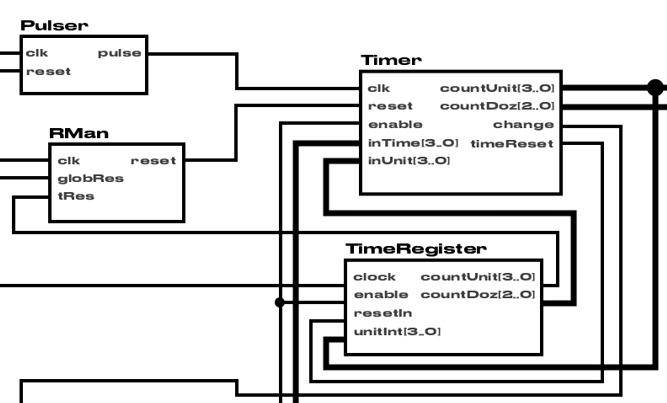
\includegraphics[width=10cm]{controlo_de_tempo.png}
	\caption{Sistema de controlo de tempo \\}
	\label{fig:time_control}
\end{figure} 
	

%%%%%
\section{Fase 3}
\label{sec.fase3}

Nesta fase, foi possível a integração das fases anteriores \autoref{sec.fase1} e \autoref{sec.fase2}, ie, integração da \acf{mef} com o sistema de controlo de tempo \autoref{fig:time_control}, cuja funcionalidade foi testada de forma adequada.


%%%%%
\section{Fase 4}
\label{sec.fase4}

Nesta fase, foi criado uma funcionalidade de paragem da \acf{mlr}. Para esse efeito foi implementado um sinal \textit{"inStart"} que dita se o processo de lavagem deve ser parado, contudo, não terminando o programa, sendo que caso seja ativado novamente, o processo (operação) do programa selecionado reinicia nas mesmas condições antes de ter sido parado.  

%%%%%
\section{Fase 5}
\label{sec.fase5}

Nesta fase, foi projetada e implementada a interface de sinais de \textit{display} que indicam o estado de funcionamento da máquina, tempo decorrido, paragem de sistema e indicações de paragem ou finalização de programa selecionado. Para esse efeito usamos componentes anteriormente indicados no \autoref{chap.arquitetura} na \autoref{sec.comp}, nomeadamente os componentes: 

\begin{itemize}

	\item\textbf{Bin7SegDec\_Timer:} Indica o tempo decorrido em segundos para cada operação do estado atual da \ac{mef}. Esta indicação é feita em sistema numérico \textbf{decimal}, e executada em dois \textit{displays} binários de 7 segmentos. Em caso de paragem da \acf{mlr} por ativação de botão \textit{inStart}, referido na \autoref{sec.fase4}, este display apresenta um sinal "\textbf{\textit{=}}".
	
	
	\item\textbf{Bin7SegDecProg:} Indica a letra \textbf{P} (para "Programa") e indica o número do programa selecionado (P1, P2 ou P3). Esta indicação é feita em sistema numérico \textbf{decimal}, e executada em dois \textit{displays} binários de 7 segmentos. Caso a entrada/função \textit{inStart} esteja desativada, a letra \textbf{P} será apagada.
	
\end{itemize}


\begin{figure}[H]
	\centering
	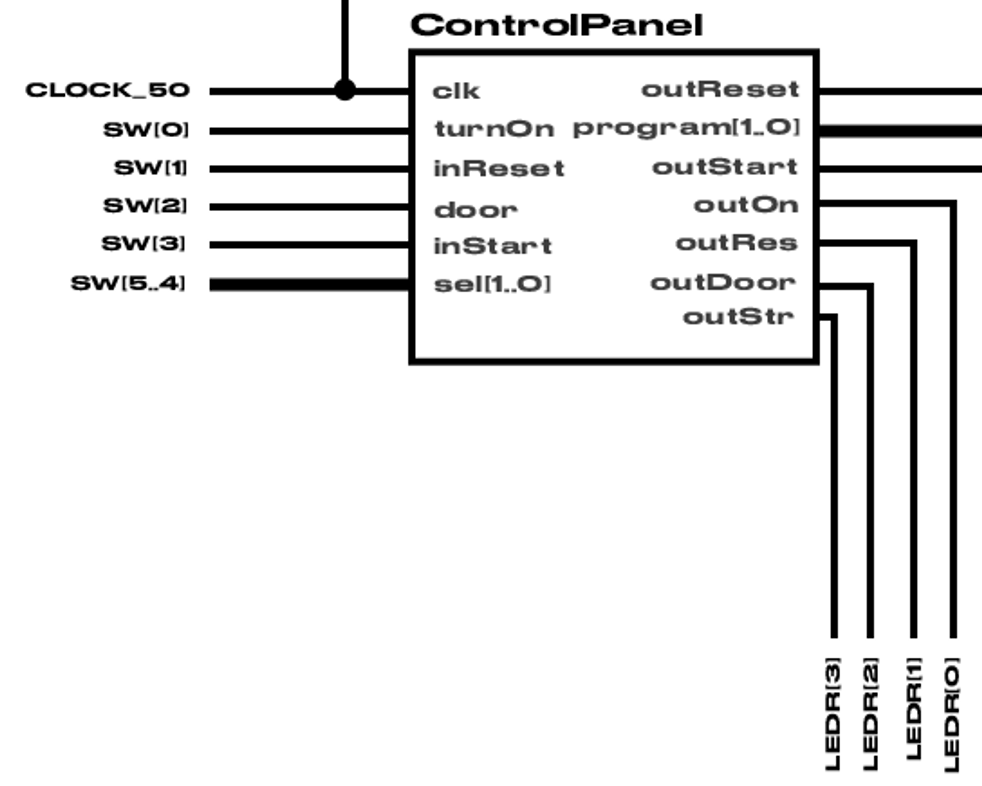
\includegraphics[width=10cm]{ControlPanel.png}
	\caption{Componente ControlPanel \\}
	\label{fig:control_panel}
\end{figure} 

\begin{figure}[H]
	\centering
	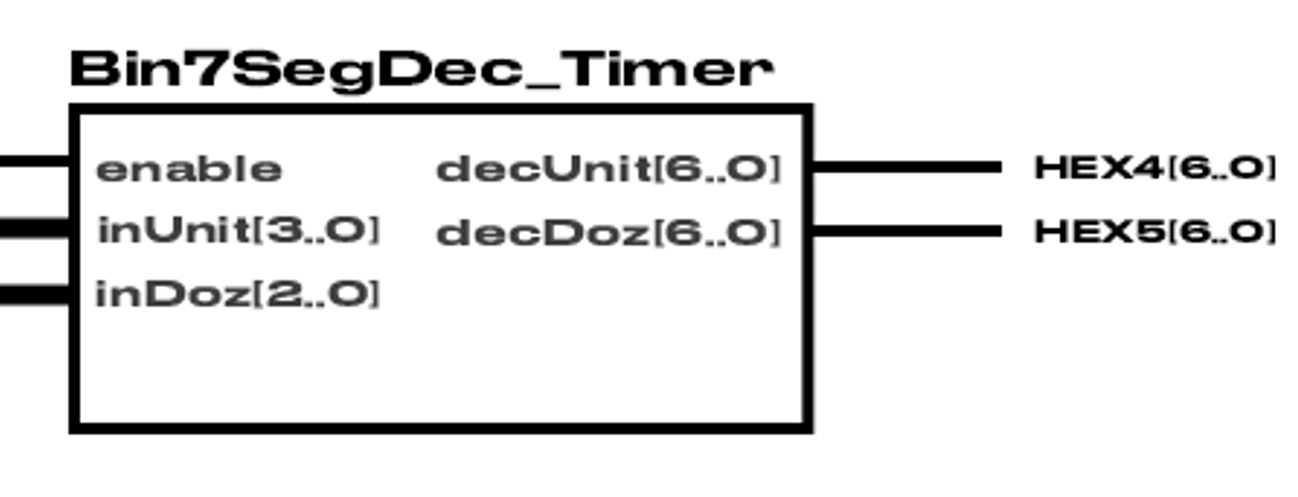
\includegraphics[width=10cm]{Bin7SegDec_Timer.png}
	\caption{Componente Decoder Binário de 7 Segmentos para Display de tempo. \\}
	\label{fig:bin7segdec_timer}
\end{figure} 

\begin{figure}[H]
	\centering
	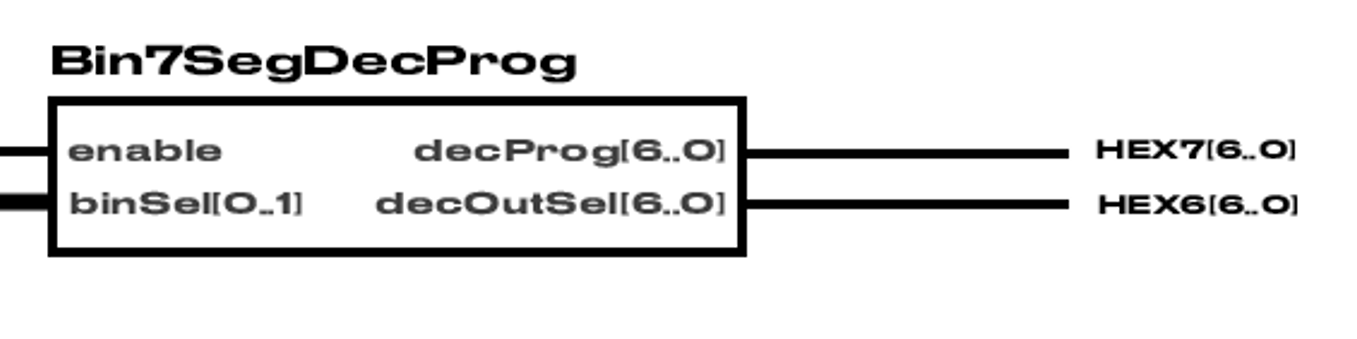
\includegraphics[width=10cm]{Bin7SegDecProg.png}
	\caption{Componente Decoder Binário de 7 Segmentos para Display de programa selecionado. \\}
	\label{fig:bin7segdecprog}
\end{figure} 
	
  

%%%%%
\section{Fase 6}
\label{sec.fase6}

Nesta fase foi executada a integração total da interface do sistema, tendo sido criando um ficheiro \ac{vhdl} \textit{"top-level"}, onde foram instanciados todos os componentes criados e delineados os sinais de ligação entre os mesmos.

\begin{figure}[H]
	\centering
	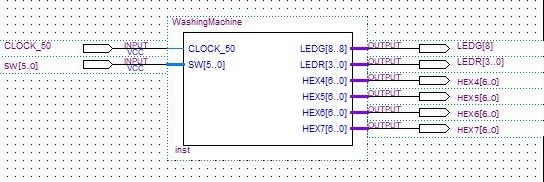
\includegraphics[width=15cm]{WashingMachineMainBlock.jpg}
	\caption{Representação bloco geral do Top-level desenvolvido em \ac{vhdl}. \\}
	\label{fig:top_level}
\end{figure} 


%%%%%
\section{Fase 7}
\label{sec.fase7}

A fase 7 pretendia a integração de uma função de inicialização diferida (temporal) pela \ac{mef}. Contudo, a mesma não foi implementada por razões indicadas na \autoref{chap.conclusão}.

%%%%%%%%%%%%%%%%%%%%%%%%%%%%%%%%%%%%%%%%%%%%%%%%%%%%%%%%%
%%%%%CAPÍTULO 3: Validação

\chapter{Validação}	
\label{chap.validação}
\lhead{Validação}

A validação foi concretizada após a realização de toda a implementação e consequentemente a especificação dos requisitos funcionais. Deste modo, foi realizadas várias \emph{testbenchs} de modo a poder averiguar se existiram possíveis erros no código escrito no projeto desenvolvido, permitindo a sua correção atempadamente. \\ 
Ao mesmo tempo, e de forma a poder controlar mais cada passo dado na realização do projeto, foi-se também testando as funcionalidades conseguidas na \ac{fpga}.
Deste modo, seguem-se as imagens resultantes de \textit{testbenches} realizadas que comprovam o bom  funcionamento dos blocos presentes na arquitetura do sistema digital desenvolvido:

\begin{figure} [H]
\centering
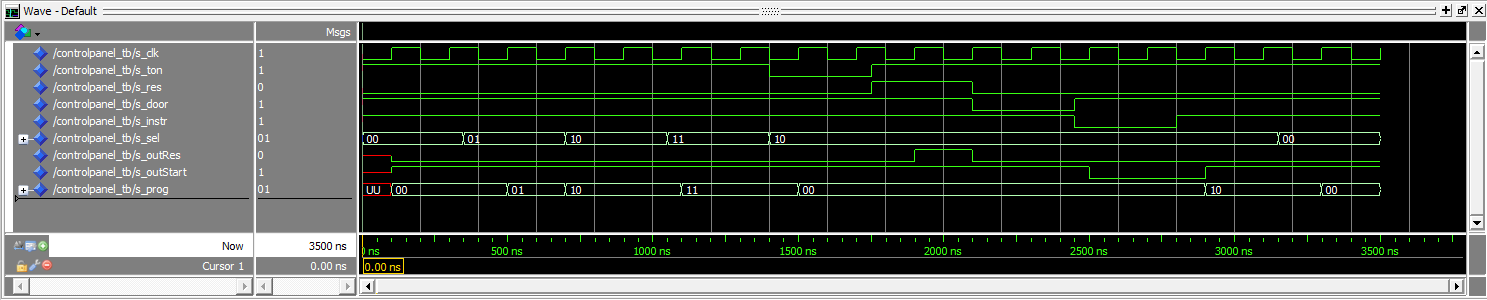
\includegraphics[width=15cm]{Testbench_ControlPanel.png}
\caption{Testbench do \textit{Control Panel}}
\label{fig:test_controlPanel}
\end{figure}

\begin{figure} [H]
\centering
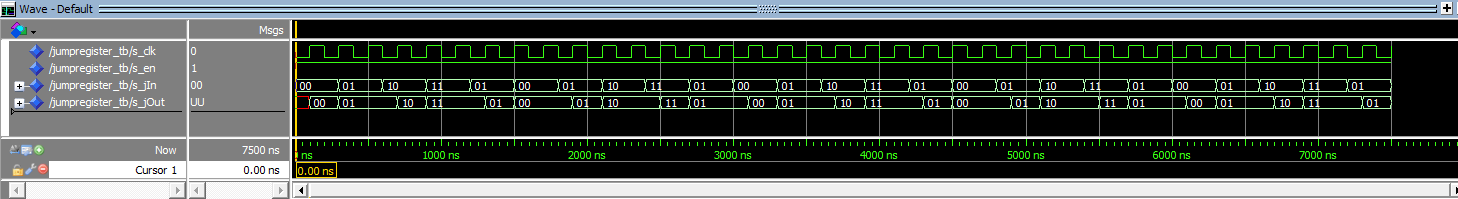
\includegraphics[width=15cm]{Testbench_JumpRegister.png}
\caption{Testbench do \textit{Jump Register}}
\label{fig:test_controlPanel}
\end{figure}

\begin{figure} [H]
\centering
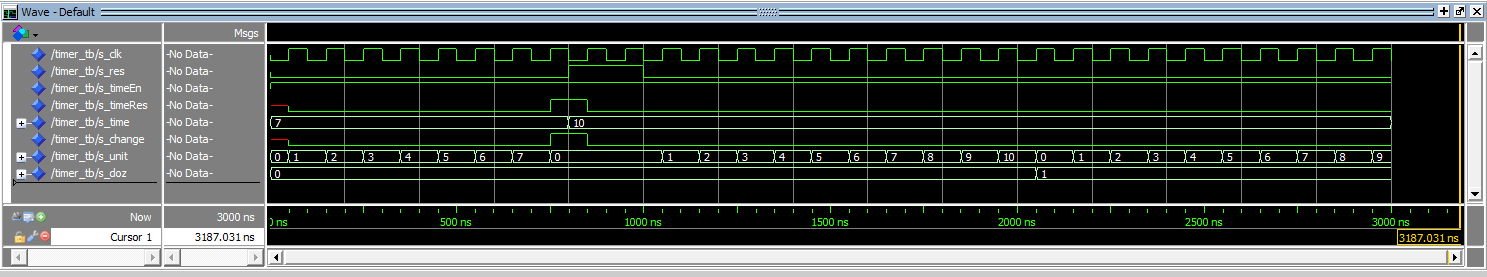
\includegraphics[width=15cm]{Testbench_Timer.png}
\caption{Testbench do \textit{Timer}}
\label{fig:test_controlPanel}
\end{figure}

\begin{figure} [H]
\centering
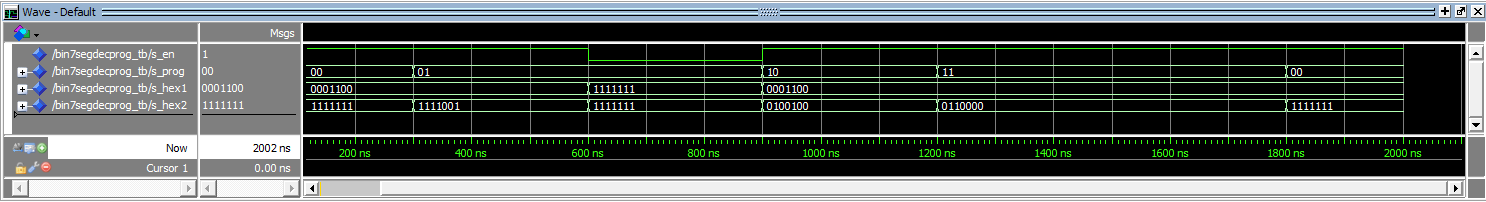
\includegraphics[width=15cm]{Testbench_Bin7SegDecProg.png}
\caption{Testbench do \textit{Display} de 7 segmentos que demonstra o programa selecionado}
\label{fig:test_controlPanel}
\end{figure}

\begin{figure} [H]
\centering
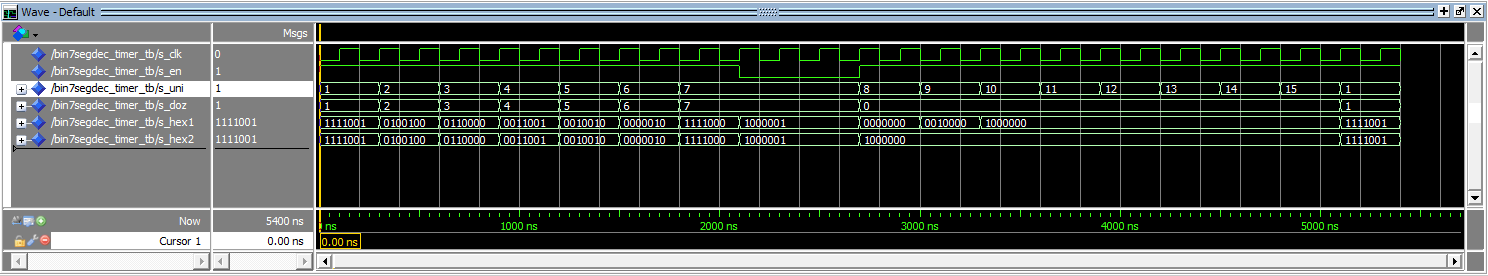
\includegraphics[width=15cm]{Testbench_Bin7SegDec_Timer.png}
\caption{Testbench do \textit{Timer} exibido no \textit{Display} de 7 segmentos}
\label{fig:test_controlPanel}
\end{figure}


%%%%%%%%%%%%%%%%%%%%%%%%%%%%%%%%%%%%%%%%%%%%%%%%%%%%%%%%%
%%%%%CAPÍTULO 4: Manual de Utilizador

\chapter{Manual de Utilizador}	
\label{chap.manual}
\lhead{Manual de Utilizador}

\section{Programas de lavagem disponíveis}
\label{sec.programas}

\begin{enumerate}
	\item\textbf{P1 - Lavagem completa:} Ao iniciar, é colocada água com uma duração de 7 segundos, procede-se o enxaguamento que obtém uma duração de 10 segundos e tira-se a água durante 4 segundos. Todo este processo é repetido outra vez, sendo que posteriormente realiza-se um \emph{spin}, tira-se novamente a água e chega-se ao estado final que não permite que a porta seja aberta por 2 segundos. Todo o processo conta com uma duração total de 53 segundos.
	

	\item\textbf{P2 - Pré Lavagem:} Após depositar a água, durando 7 segundos, realiza-se o enxaguamento, que por si dura 10 segundos, e tira-se a água que havia sido depositada anteriormente durante 4 segundos. De seguida, da-se a ocorrência de um \emph{spin} por 5 segundos e consequentemente a tiragem da água por 4 segundos. Este processo conta com uma duração total de 32 segundos.


	\item\textbf{P3 - Extra-spin:} Depois de realizado o pedido de extra-spin, dá-se o \emph{spin} por 5 segundos, tira-se a água por 4 segundos e chega-se ao estado final que impossibilita a abertura da porta por 2 segundos.
\end{enumerate}


\begin{figure}[H]
	\centering
	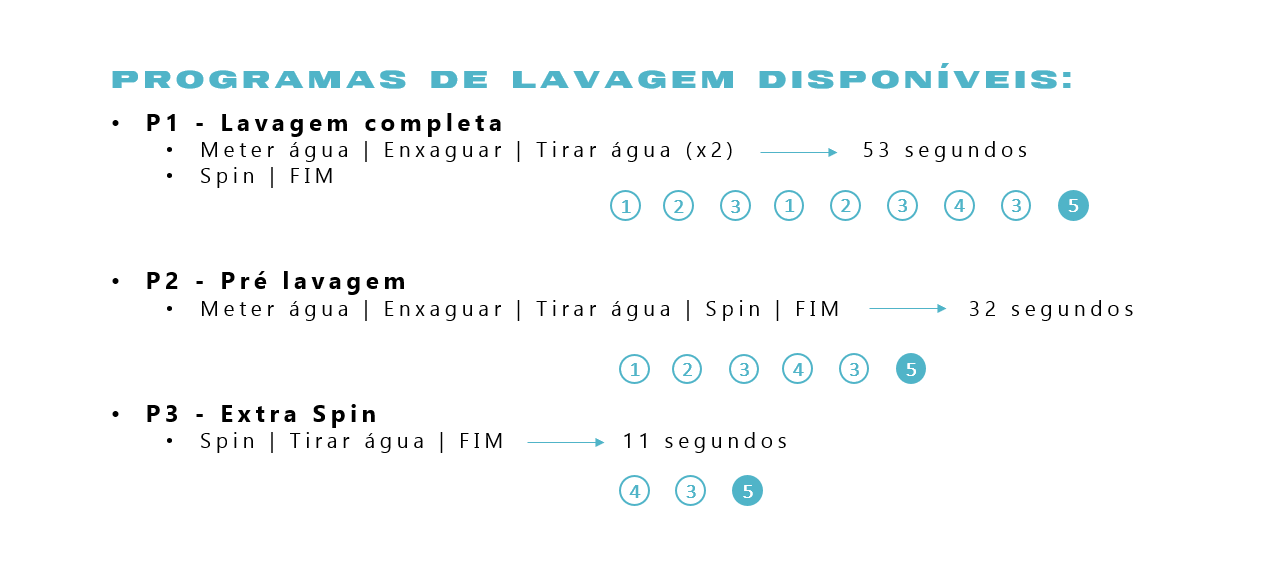
\includegraphics[width=15cm]{Programas.png}
	\caption{Instruções: Programas de lavagem}
	\label{fig:programas}
\end{figure}


\section{Interface}
\label{sec.interface}

\subsection{Botões de Interação}
\label{sec.botões}

Para utilizar a \acf{mlr} deve primeiro familiarizar-se com os seus botões principais:

\begin{enumerate}
	\item\textbf{Botão ON/OFF - (SW0):} Este botão permite ligar a \ac{mlr}. Caso esteja desligado, a sua máquina não irá funcionar.
	\item\textbf{Botão Reiniciar - (SW1):} Este botão permite reiniciar a sua máquina em caso de introdução equivoca de um programa não desejado. Deve ser ativado só se pretender reiniciar a sua máquina.
	\item\textbf{Botão de Porta - (SW2):} Este botão permite abrir e fechar a porta da sua máquina. A porta deve estar sempre fechada, pois caso contrário e para sua segurança a sua máquina não irá iniciar qualquer programa selecionado.	
	\item\textbf{Botão Start - (SW3):} Este botão permite iniciar o programa de lavagem que selecionou da lista de programas disponíveis em \autoref{sec.programas}. 
	
\end{enumerate}
		
Sobre os botões referidos, existem na máquina luzes de aviso para indicar se cada um deles está  corretamente acionado. Caso um dos botões não esteja numa posição válida que impeça a iniciação de um programa, a luz de aviso sobre o botão que necessita da sua atenção irá apagar-se, indicando que a máquina não se encontra preparada para iniciar, tal como demonstrado na figura seguinte:

\begin{figure}[H]
	\centering
	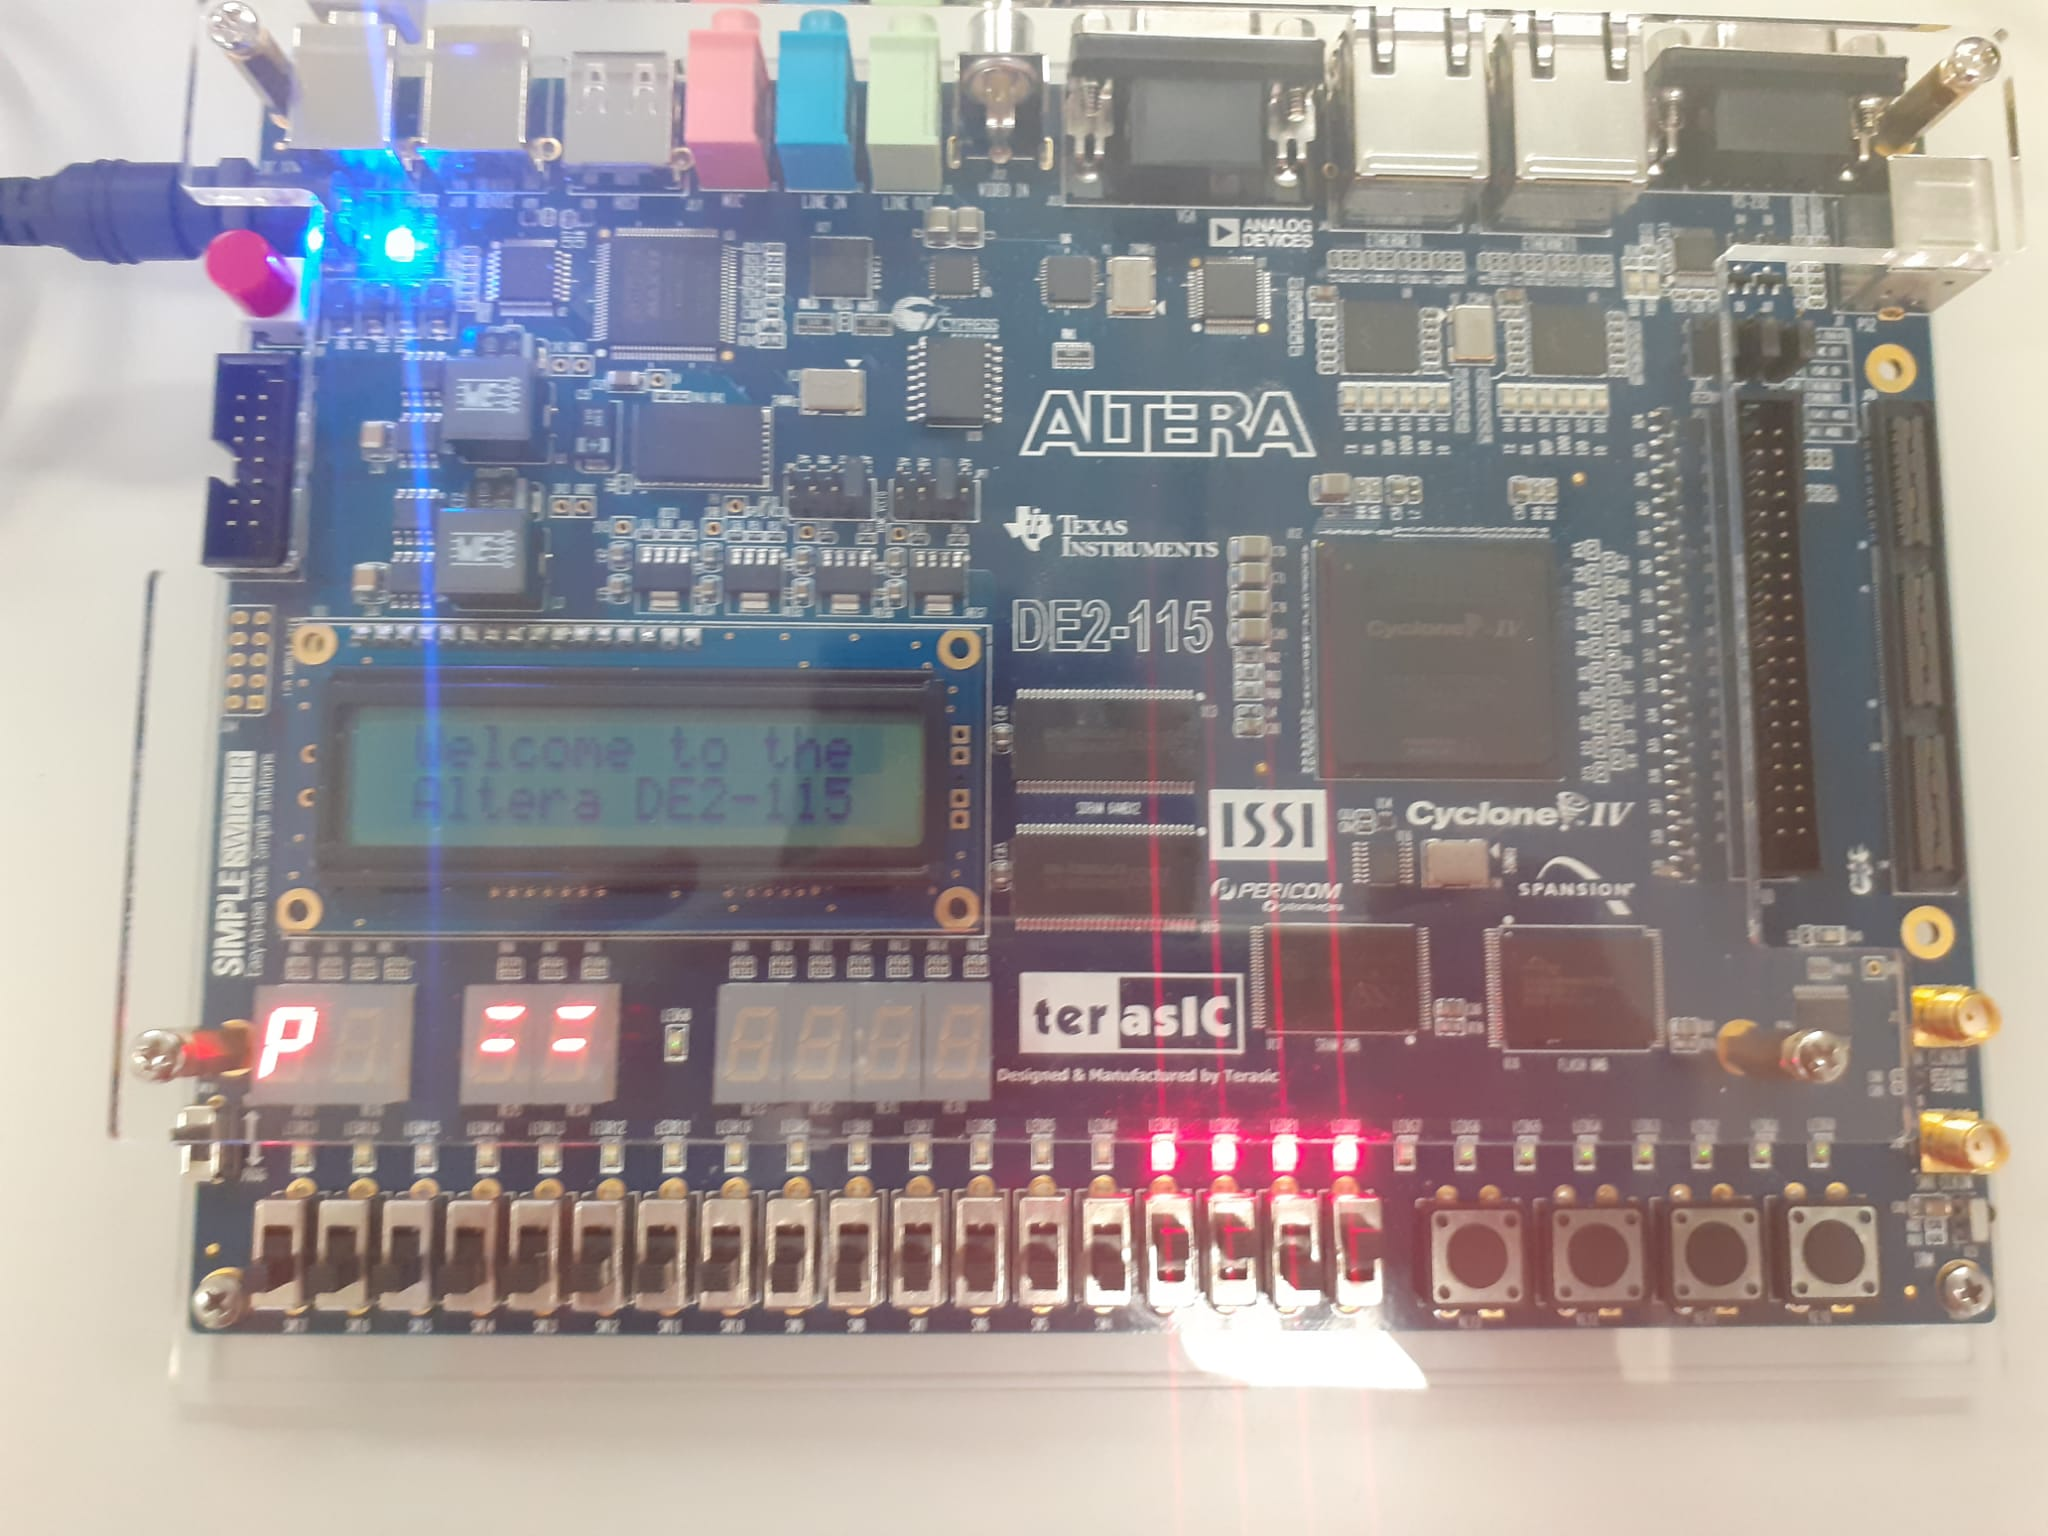
\includegraphics[width=15cm]{luzes_aviso.jpeg}
	\caption{Luzes de aviso.}
	\label{fig:botoes_sistema}
\end{figure}


	\begin{itemize}
	\item\textbf{Botões de seleção de programa - (SW4 e SW5):} Estes botões permite-lhe selecionar o programa que deseja: 
	\begin{enumerate}
		\item Caso pretenda o Programa Nº1 \textit{"Lavagem Completa"}, deve ativar apenas o botão SW4. 
		\item Caso pretenda o Programa Nº2 \textit{"Pré-lavagem"}, deve ativar ambos os botões.
		\item Caso pretenda o Programa Nº3 \textit{"Extra-Spin"}, (ie, Centrifugação-Extra) deve ativar apenas o botão SW5. 
	\end{enumerate}	
	\end{itemize}		
		
\begin{figure}[H]
	\centering
	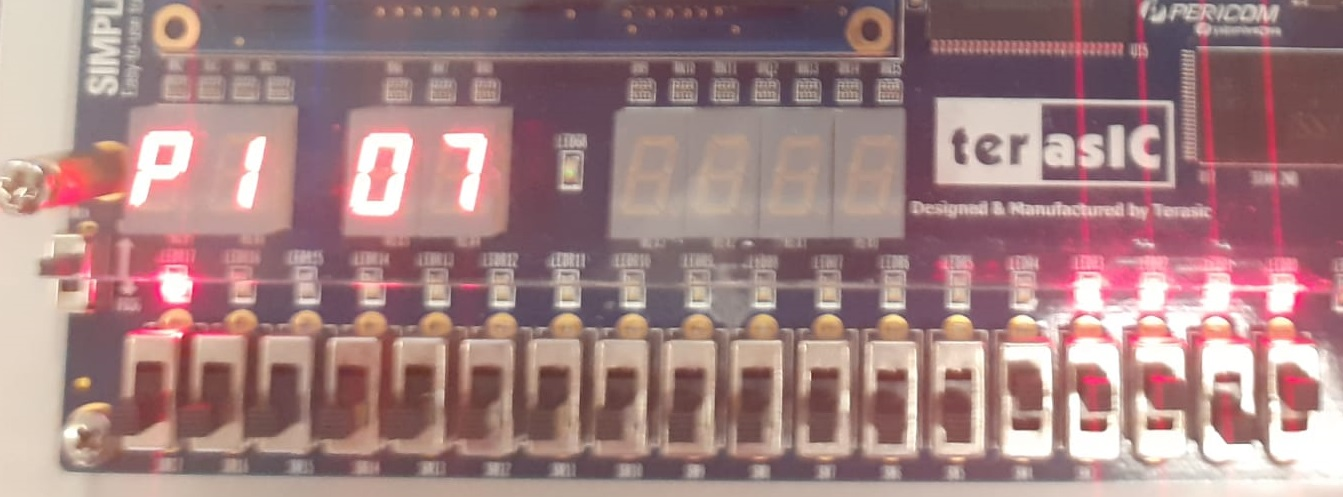
\includegraphics[width=15cm]{demo.jpeg}
	\caption{Instruções: Botões Principais da \acf{mlr}}
	\label{fig:interface}
\end{figure}

\subsection{Displays de Informação}
\label{sec.display}

Para finalizar, iremos falar sobre os \textit{displays} e o significado das mensagens de cada um deles, fazendo recurso de um cenário de demonstração exemplar prática. Na figura \autoref{fig:interface}, do lado esquerdo pode verificar que existem 4 \textit{displays} de 7 segmentos, onde o mais à esquerda indica a letra \textbf{P} e os restantes 3(três) indicam números. \\ 
A letra \textbf{P} indica que a sua máquina encontra-se pronta em modo \textit{START} e requer a escolha de um programa. Caso tenha selecionado um programa (por exemplo, Programa Nº 3) o \textit{display} imediatamente ao lado da letra \textbf{P} irá indicar o número do programa que escolheu. \\
Os restantes 2(dois) \textit{displays} apresentam o tempo decorrido em cada funcionalidade da máquina tal como descrito na \autoref{sec.programas}. Caso os displays temporais apresentem um sinal "\textbf{=}", significa que a sua máquina encontra-se em \textit{standby}, por desativação do botão \textit{Start} (funcionalidade STOP). Este símbolo pode aparecer ainda momentaneamente quando a sua máquina terminar um processo no decorrer do programa selecionado.\\

Existem ainda 4 luzes imediatamente a baixo dos displays - Luzes LEDR(17), LEDR(16), LEDR(15) e LEDR(14). Quando cada uma destas luzes se encontra acionada (acesa), significa que a sua máquina está a executar uma funcionalidade especifica, tal como indicado na tabela a baixo:


\begin{table}[H]
    \centering
    \caption{Luzes de Funcionalidade.}
    \begin{tabular}{|c|c|c|}\hline

        Funcionalidade 			& Luz acionada	\\ 
        \hline
	    Meter água 				& LEDR(17)		\\
	    Enxaguar			 	& LEDR(16) 		\\
	    Remover água 			& LEDR(15)		\\ 
		Centrifugação 			& LEDR(14		\\
				
    \hline
    \end{tabular}
    \label{tab.luzes_funcao}
\end{table}	


O cenário exemplar descrito a cima pode ser contemplado na figura seguinte:

\begin{figure}[H]
	\centering
	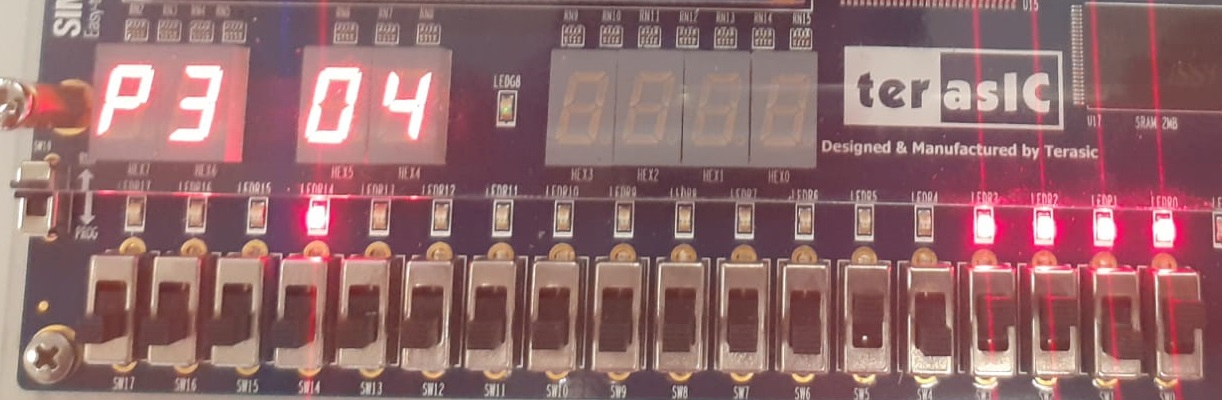
\includegraphics[width=15cm]{interface.jpeg}
	\caption{Instruções: displays e sinais luminosos da \acf{mlr}}
	\label{fig:interface}
\end{figure}



%%%%%%%%%%%%%%%%%%%%%%%%%%%%%%%%%%%%%%%%%%%%%%%%%%%%%%%%%
%%%%%CAPÍTULO 5: CONCLUSÃO
%

\chapter{Conclusão}
\label{chap.conclusão}
\lhead{Conclusão}

Este documento visa relatar todo o desenvolvimento desde o planeamento, sintetização, modelação e validação do sistema digital desenvolvido sob forma de projeto final à unidade curricular de Laboratórios de Sistemas Digitais no ano letivo de 2021/2022.\par
Deste modo é viável afirmar que o trabalho realizado correspondeu aos objetivos definidos, sendo possível criar diversos componentes importantes para o seu desenvolvimento cujas \textit{testbenches} e testes executados foram positivos e implementação destes num ficheiro \textit{top-level} configurável na \ac{fpga}. Nem sempre foi possível implementar as ideias concebidas inicialmente, contudo esteve sempre presente a capacidade de adaptação face às adversidades obtidas no desenvolver do projeto.\par 
Apenas a \autoref{sec.fase7} não foi possível desenvolver, devido à dificuldade de implementar tendo por base o sistema que já criado.\par
Este projeto foi desenhado de modo a que o utilizador possa interagir com a interface numa forma mais intuitiva, onde o \emph{output} direcionado tanto aos \emph{LED's} como aos \emph{displays} demonstram distintas e visíveis diferenças aquando dos diferentes pedidos realizados.\par
Em suma, afirma-se que foi o projeto final foi ao encontro às metas estabelecidas, e por essa razão considera-se que o mesmo foi bem sucedido.

%
%%%%%%%%%%%%%%%%%%%%%%%%%%%%%%%%%%%%%%%%%%%%%%%%%%%%%%%%%
%%%%%CONTRIBUIÇÕES DE AUTORES:
% 
\chapter*{Contribuições dos Autores}

\begin{table}[H]
    \centering
    \caption{Contribuições dos Autores.}
    \begin{tabular}{|c|c|c|c|}\hline

        Contribuição 			& João Vieira 	& Leandro Costa  	\\ 
        \hline
	    Produção de Relatório 	& 50~\% 		& 50~\%	    	 	\\
	    Produção PowerPoint 	& 10~\% 		& 90~\%  			\\
	    Produção Vídeo 			& 10~\% 		& 90~\% 			\\ 
		Produção VHDL 			& 100~\% 		& 0~\%				\\
		Testbenches 			& 100~\% 		& 0~\%				\\
		Testing e Validação 	& 85~\% 		& 15~\% 			\\
		Correção de erros VHDL	& 85~\% 		& 15~\% 			\\		
		
    \hline
    \end{tabular}
    \label{tab.contribuições}
\end{table}	

%
%%%%%%%%%%%%%%%%%%%%%%%%%%%%%%%%%%%%%%%%%%%%%%%%%%%%%%%%%
%%%%%BIBLIOGRAFIA:
%
\begin{thebibliography}{9}

\bibitem{enunciado7} 
Laboratórios de Sistemas Digitais -
\textit{Enunciado Nº7 - Máquina lavagem de roupa}. |
Universidade de Aveiro, LSD, versão 1, 2021/22


\bibitem{de2-115} 
ALTERA -
\textit{DE2-115 User Manual}. |
Terasic Technologies Inc, Copyright 2003-2010


\end{thebibliography}
\end{document}
